\documentclass[12pt]{article}

%\ifx\pdfoutput\undefined
\usepackage{graphicx}
%\else
%\usepackage[pdftex]{graphicx}
%\fi

\usepackage[utf8]{inputenc}
\usepackage[english,russian]{babel}
\usepackage{mathtext}
%\usepackage{misccorr}%ставит точки после теорем
\usepackage{indentfirst}
\usepackage{paralist}
\usepackage{geometry}
\usepackage{cmap}
\usepackage{amsthm}
%\usepackage{comment}
%\usepackage{colon}
\usepackage{setspace}
\onehalfspacing

\newtheorem{theorem}{\hspace{1cm}Теорема}
\newtheorem{lemma}{\hspace{1cm}Лемма}
\newtheorem{result}{\hspace{1cm}Следствие}

 \geometry{verbose,a4paper,tmargin=1.5cm,% bmargin=2cm,
 	  lmargin=3.5cm %,rmargin=1.5cm
 }

\usepackage{indentfirst} % Красная строка после заголовка
\setlength\parindent{1cm} % 
 
 
\begin{document}
	
	
	\begin{titlepage}
		\thispagestyle{empty}
		\begin{center}
			{
				Министерство образования и науки Российсской Федерации\\
				Федеральное государственное бюджетное образовательное учреждение\\
				высшего образования\\
				\textbf{ <<Омский~государственный~университет~им.~Ф.~М.~Достоевского>>\\
					Институт математики и информационных технологий\\
					Кафедра прикладной и вычислительной математики\\[3.0cm] }
			}
			
			\textbf{\Large Исследование наследственного класса рёберных графов двудольных графов\\[10pt]}
			
			Выпускная квалификационная работа\\
			по направлению подготовки специалистов\\
			01.05.01 Фундаментальные математика и механики\\[2.0cm]
			
			\begin{flushright}
				\begin{minipage}{0.4\textwidth}
					Выполнил:\\
					студент группы МАС-301-О\\
					Горбунов Никита Викторович\\[8pt]
					\hrule \par\smallskip
					{\it (подпись студента)}\\[10pt]
					Научный руководитель:\\
					д.ф.-м.н., профессор\\
					Ильев Виктор Петрович\\[8pt]
					\hrule \par\smallskip
					{\it (подпись руководителя)}
				\end{minipage}
			\end{flushright}
			
			\vfill
			\vspace{7mm}
			{\large Омск 2018}
			
		\end{center}
	\end{titlepage}
	
	
	
\large

%_________________________________________________________________________________________________________

\textwidth = 160mm
\textheight = 240mm

%_________________________________________________________________________________________________________


\newpage

\tableofcontents % Вывод содержания

\newpage
\begin{center}
%	\section*{Исследование наследственного класса рёберных графов двудольных графов}
	\section*{Введение}
\end{center} 
	

Целью дипломной работы является исследование наследственных классов графов в терминах запрещённых подграфов. Особое внимание уделено исследованию наследственного класса рёберных графов двудольных графов.

Актуальность темы дипломной работы объясняется тем, что исследуемый класс рёберных графов нашёл применение в доказательстве "Cильной теоремы о совершенных графах". В 1963 году в статье  Бержа была высказана гипотеза об эквивалентности классов совершенных графов и графов Бержа. Гипотеза была доказана в 2002 году, как "Сильная теорема о совершенных графах"\ и опубликована в 2006 году М.Чудновской, Н.Робертсоном, П.Сеймуром и Р.Томасом [8].

Кроме того, рёберные графы двудольных графов играют важную роль в характеризации графов баз матроидов [10].

Пусть $G=(V,E)$ и $ G'=(V',E')$ -- неориентированные графы. Графы $G$ и $G'$ называются {\it изоморфными}, если существует биекция $\varphi : V \to V'$, такая, что $xy \in E \Leftrightarrow \varphi(x)\varphi(y) \in E'$ при всех $ x,y \in V$. Если $ V' \subseteq V$ и $E' \subseteq E$, то $G'$ называется {\it подграфом} графа $G$, обозначается $G' \subseteq G$.

Множество графов, замкнутое относительно изоморфизма, называется {\it классом} графов.

Если $G' \subseteq G$ и $G'$ содержит все рёбра $xy \in E$ при $x,y \in V'$, то $G'$ -- {\it порождённый} подграф $G$.

Класс графов, замкнутый относительно операции удаления вершин, называется {\it наследственным}. Иначе этот класс может быть определён в терминах запрещённых порождённых подграфов.

Если $X$ класс графов, то через {\it Forb(X)} обозначается класс всех графов, не содержащих порождённых подграфов, изоморфных графам из $X$. Графы из $X$ называются {\it запрещёнными} порождёнными подграфами. Верен следующий критерий наследственности класса графов. Аналогичное утверждение для случая  миноров можно найти в книге Дистеля [4].

\begin{theorem}
\label{t1}
Класс графов $Y$ является наследственным классом тогда и только тогда, когда $Y = Forb(X)$ для некоторого $X$.
\end{theorem} 
% Класс графов $Y$ является наследственным классом тогда и только тогда, Y не содержит порождённых подграфов, изоморных графам некоторого Х.
\vspace{-3mm}

Наследственный класс графов называется {\it монотонным}, если он замкнут относительно операций удаления вершин и рёбер. Иначе он может быть определён в терминах запрещённых подграфов, необязательно порождённых.

\vspace{-3mm}
\begin{theorem}
\label{t2}	
	Класс графов Y является монотонным наследственным тогда и только тогда, когда Y не содержит подграфов, изоморфных графам некоторого класса $X$.
\end{theorem}
\vspace{-3mm}

Запрещённый порождённый подграф является {\it минимальным}, если при удалении любой вершины он перестаёт быть запрещённым.
Запрещённый подграф является {\it минимальным}, если при удалении любой вершины или ребра он перестаёт быть запрещённым.

В данной дипломной работе будут рассмотрены примеры наследственных классов графов, дано их описание через запрещённые подграфы. 

В параграфе 1 приведены минимальные запрещённые подграфы для основных классов графов. В параграфе 2.1 подробнее рассмотрены рёберные графы. В параграфе 2.2 даётся введение в класс рёберных графов двудольных графов. В параграфе 2.3  найдены запрещённые подграфы для класса рёберных графов двудольных графов.

Далее будут рассматриваться только {\it обыкновенные графы}, т.е. графы без петель и кратных рёбер.
%\section{\centerline{ Основные определения и факты}}
%%%%%%%%%%%%%%%%%%%%%%%%%%%%%%%%%%%%%%%%%%%%%%%%%%%%%%%%%%%%%%%%%%%%%%%%%%%%%%%%%%%%%%%%%%%%%%%%%%%%%%%%%%%%%%%%%%%%%%%%%%%%%%%%%%%%%%%%%%%%%%%%%%%%%%%%%%%%%%%%%%%%%%%%%%%%%%%%%
\newpage

\section{Примеры наследственных классов графов}


\subsection{Леса}
Граф называется {\it ациклическим}, если в нём нет циклов. {\it Дерево} -- это связный ациклический граф. Каждый граф, не содержащий циклов, называется {\it лесом} (рис. 1).

{\it Маршрутом} в графе $G$ называется чередующаяся последовательность вершин и рёбер $v_0, e_1, v_1, ... , v_{n-1}, e_n, v_n$ такая, что $e_i=v_{i-1}v_i$ для любого $i$. %эта последовательность начиначется и кончается вершиной, и каждое ребро последовательности инцидентно двум вершинами, одна из которых непосредственно предшествует ему, а другая непосредственном следует за ним.%
{\it Простой цепью} в графе $G$ называется маршрут, в котором все вершины различны. Простая цепь с $n$ вершинами обозначается $P_n$.
Замкнутая цепь называется {\it циклом}. Замкнутый маршрут называется {\it простым циклом}, если все его $n$ вершин различны и $n \geq 3$. Простой цикл с $n$ вершинами обозначается $C_n$.

Класс всех лесов является монотонным наследственным классом графов. Минимальными запрещёнными подграфами в классе лесов являются простые циклы.

\begin{figure}
\begin{center}
	\label{pic1}
	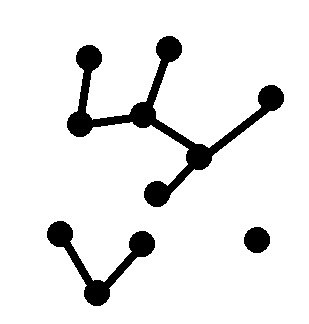
\includegraphics[scale=0.33]{les.jpg}
	\caption{Лес}
\end{center}
\end{figure}
\vspace{-3mm} 
\subsection{Двудольные графы} 
 Граф $G = (V,E)$ называется {\it двудольным}, если $V$ допускает такое разбиение на два подмножества $V_1$ и $V_2$ ({\it доли}), при котором концы каждого ребра лежат в разных долях (рис. 2). Если каждая вершина множества $V_1$ смежна с каждой вершиной из множества $V_2$, то такой граф называется {\it полным двудольным}. Если при этом множество $V_1$ содержит $m$ вершин, а множество $V_2$~-- $n$ вершин, то такой граф обозначается $K_{m,n}$. {\it Звездой} называется полный двудольный граф $K_{1,n}$. 
 
 Класс двудольных графов является монотонным наследственным классом. Минимальными запрещеными подграфами в классе двудольных графов являются все простые циклы нечётной длины. Последнее верно в силу следующего известного критерия двудольности графа.

\begin{theorem}[Кёниг]
	\label{t3}
Граф двудолен, если и только если он не содержит циклов нечётной длины.
\end{theorem} 
\vspace{-3mm}
Доказательство данного критерия можно найти в книге \\Ф.Харари~[5].

\begin{figure}
\begin{center}
	\label{pic2}
	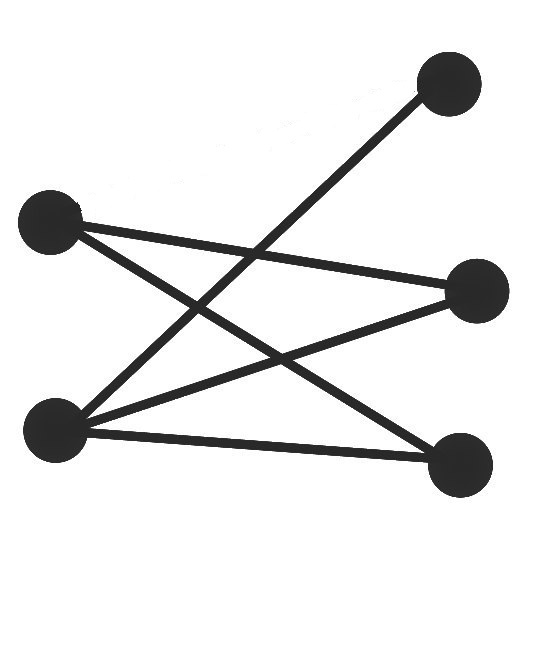
\includegraphics[scale=0.22]{dvud.jpg}
	\caption{Двудольный граф}
\end{center}
\end{figure}

\vspace{-5mm}

\subsection{Клики }
{\it Регулярный граф} -- граф, степени всех вершин которого равны. {\it Пустым графом} называется регулярный граф степени 0, то есть граф без рёбер. Обозначается $O_n$, где $n$ -- количество вершин.
{\it Клика } -- полный граф (рис. 3). Клика с $n$ вершинами обозначается $K_n$. Класс всех клик является наследственным классом. Единственным минимальным запрещённым порождённым подграфом для класса клик является пустой двухвершинный граф $O_2$.
\\

\begin{figure}
	\label{pic3}
	\centering{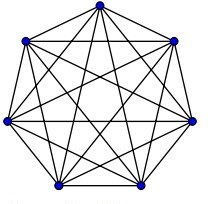
\includegraphics[scale=0.5]{klicka.jpg}}
	\caption{Клика $K_7$}
\end{figure}

\vspace{-5mm}

\subsection{Планарные графы }
Говорят, что граф {\it укладывается} на плоскости, если его можно нарисовать на плоскости так, что никакие два его ребра не пересекаются вне вершин.

Граф называется {\it планарным}, если его можно уложить на плоскости (рис.~4).
Два графа называются {\it гомеоморфными}, если их можно получить из одного графа с помощью последовательности подразбиений рёбер (рис.~5).

\begin{figure}
	\label{pic4}
	\centering{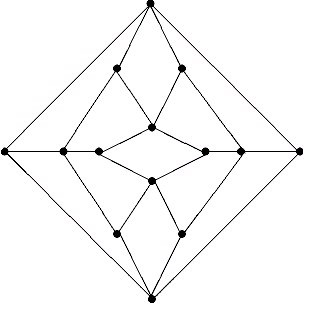
\includegraphics[scale=0.3]{planar.jpg}}
	\caption{Планарный граф}
\end{figure}

Класс планарных графов является монотонным наследственным. В следующем критерии планарности графа описаны все минимальные запрещённые подграфы для класса планарных графов.

\begin{figure}
	\label{pic5}
	\centering{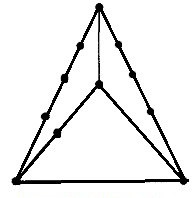
\includegraphics[scale=0.38]{gomeomorf.jpg}}
	\caption{Граф, гомеоморфный графу $K_4$}
\end{figure}

\begin{theorem}[Понтрягин-Куратовский]
	\label{t4}
%(Понтрягин-Куратовский).
Граф планарен тогда и только тогда, когда он не содержит подграфов, гомеоморфных $K_5$ или ${K_{3,3}}$ (рис.~6).
\end{theorem} 

\begin{figure}
	\label{pic6}
	\centering{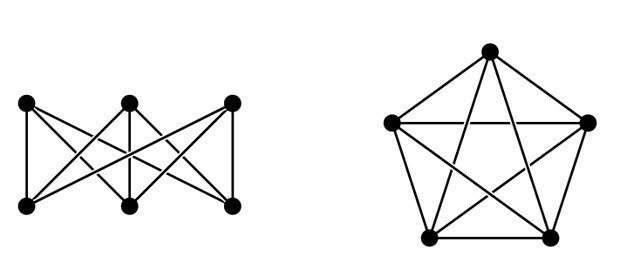
\includegraphics[scale=0.25]{k44_k5.jpg}}
	\caption{Графы $K_{3,3}$ и $K_5$}
\end{figure}
\vspace{-5mm}
\subsection{Расщепляемые графы}
Множество вершин является {\it независимым}, если никакие два его элемента несмежны.
{\it Расщепляемый} граф -- это граф, множество вершин которого можно разложить на клику и независимое множество (рис. 7).

Класс расщепляемых графов является наследственным. Минимальными запрещёнными порождёнными подграфами являются графы изоморфные $C_4, C_5$ и $K_2 \cup K_2$ (дополнение к графу $C_4$) [9].

\begin{figure}
	\label{pic7}
	\centering{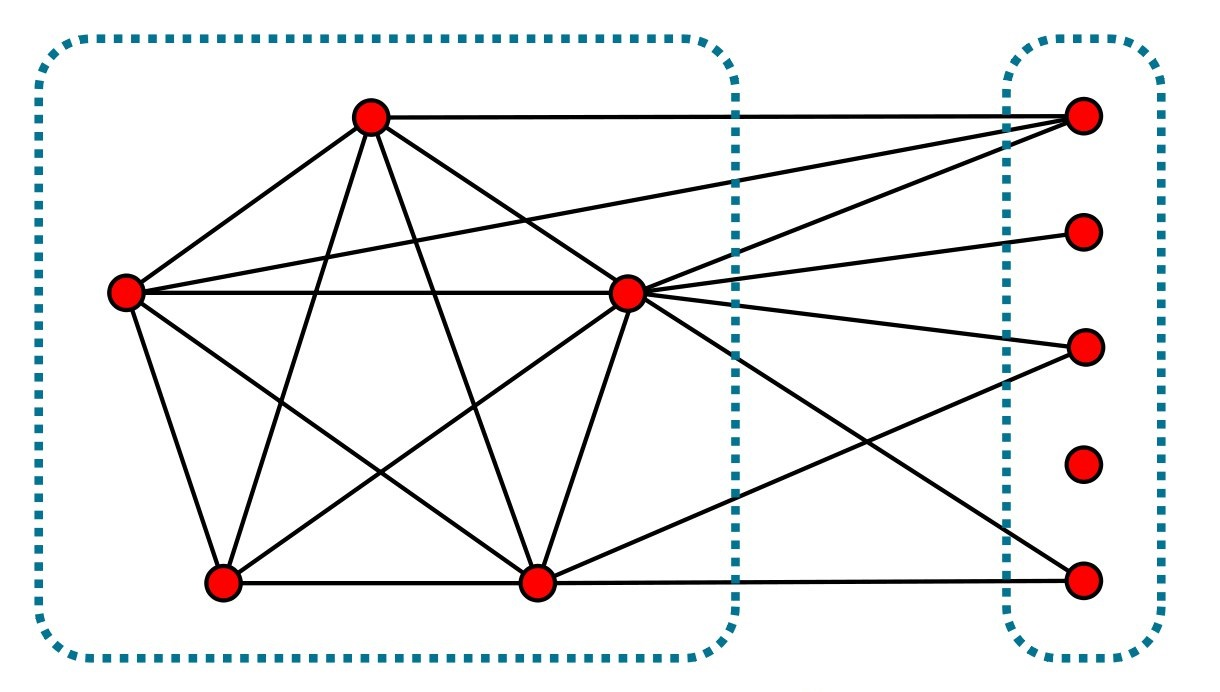
\includegraphics[scale=0.1]{raschepl.jpg}}
	\caption{Расщепляемый граф}
\end{figure}
\subsection{Кёниговы графы}
Для определения кёнигова графа нам понадобятся следующие определения.
Пусть $X$ -- множество графов на $n$ вершинах. $X$-{\it упаковкой} графа $G$ называется множество его непересекающихся порождённых подграфов, каждый из которых изоморфен какому-нибудь графу из $X$. Наибольшее число подграфов в $X$-упаковке графа $G$ обозначается через $pack(X;G)$. $X$-{\it покрытием} графа $G$ называется множество вершин, после удаления которых получается граф, не содержащий порождённых подграфов, принадлежащих $X$. Наименьшее число вершин в $X$-покрытии графа будет обозначаться через $cover(X;G)$. Граф $G$ называется {\it кёниговым графом} относительно множества $X$, если для любого его порождённого подграфа $H$ выполняется равенство $pack(X;H) = cover(X;H)$ (рис. 8).

Кёниговы графы можно определить и в терминах запрещённых подграфов [1]. Граф $G$ является кёниговым, если он не содержит порождённых подграфов из множества
$A\cup B\cup C \cup D \cup E$, где 
\\ $A$ -- множество состоящее из трёх графов: $K_1*P_4, K_1*(K_1+P_3), K_2*O_3$ ($"+"$ в данном случае просто объединение графов с непересекающимися множествами вершин, $"*"$ -- к сумме добавляются все ребра, соединяющие вершины из разных слагаемых (рис. 9));
\\ $B$ -- множество всех циклов, длина которых не кратна 3;
\\ $C$ -- множество всех графов, которые можно получить добавлением к циклу, длина которого кратна 3, двух вершин, не смежных между собой, каждая из которых соединяется ребром с одной вершиной цикла, причем расстояние между этими вершинами должно быть не кратно 3;
\\ $D$ -- множество всех графов, которые можно получить добавлением к циклу, длина которого кратна 3, двух вершин, не смежных между собой, одна из которых соединяется ребром с одной вершиной цикла, а другая с тремя подряд идущими вершинами цикла, причём расстояние между добавленными вершинами, должно быть сравнимо с 1 по модулю 3; 
\\ $E$ -- множество всех графов, которые можно получить из циклов  длины, кратной 3, путём замены 2-кликами трёх вершин цикла, разбивающих цикл на отрезки, длина каждого из которых не меньше 4 и сравнима с 1 по модулю 3.

\begin{figure}
	\label{pic8}
	\centering{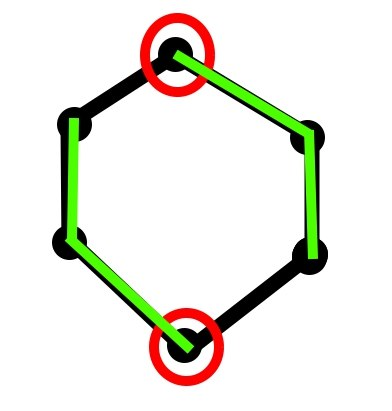
\includegraphics[scale=0.3]{Kenig_new.jpg}}
	\caption{Кенигов граф. $cover(X,H)=pack(X,H)=2$. $X=K_{1,2}$}
\end{figure}

\begin{figure}
	\centering{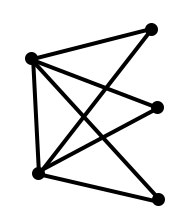
\includegraphics[scale=0.55]{umnoj.jpg}}
	\caption{$K_2*O_3$}
\end{figure}

\subsection{Блочные леса}

{\it Связным графом} называется граф, в котором любая пара вершин соединена простой цепью.
{\it Компонентой связности} графа $G$ называется максимальный связный подграф графа  $G$.
{\it Шарниром} называется вершина графа, при удалении которой количество компонент связности возрастает.
%{\it Неразделимым} графом называется связный, не пустой, не имеющий точек сочленения граф.

Связный граф, не содержащий шарниров, называется {\it блоком}.
{\it Блочный лес} -- это множество неориентированных графов, в которых каждый блок является кликой (рис. 10).
%{\it Алмазным} графом называют планарный граф с четырьмя вершинами и пятью рёбрами. Другими словами, это граф $K_4$ без одного ребра.

\begin{figure}
	\label{pic9}
	\centering{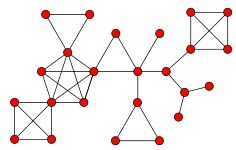
\includegraphics[scale=0.6]{block.jpg}}	
	\caption{Блочный лес}
\end{figure}

Класс блочных лесов является наследственным. Запрещёнными порождёнными подграфами в нём являются $K_4 - e$ (рис. 11) и простые циклы длины 4 и более [6].

\begin{figure}
	\label{pic10}
	\centering{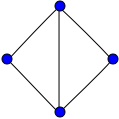
\includegraphics[scale=0.45]{diamond.png}}
	\caption{$K_4 - e$}
\end{figure}

%\subsection{Дистанционные графы}
%Дистанционный граф -- это граф изоморфный графу расстояний. Наследственный.

\newpage

\begin{center}
	\section{Рёберные графы}
	\subsection{Характеризация рёберных графов}
\end{center}

Ещё одним примером наследственного класса графов является класс рёберных графов.% Т.к. этот класс может быть определён в терминах запрещённых порождённых подграфов.

{\it Рёберным графом} 
произвольного графа $G$ называется граф $L(G)$, множество вершин которого взаимно однозначно соответствует множеству рёбер графа $G$, и две вершины в $L(G)$ смежны тогда и только тогда, когда соответствующие рёбра в $G$ имеют общую вершину (рис. 12).

Граф $G$ называется {\it рёберным графом}, если он изоморфен реберному графу $L(H)$ некоторого графа $H$.

\begin{figure}
	\label{pic11}
	\centering{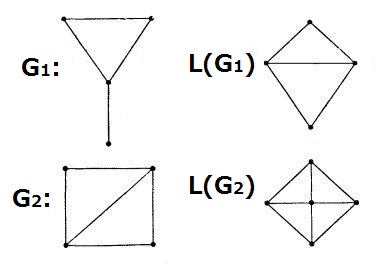
\includegraphics[scale=0.4]{reber.jpg}}
	\caption{Рёберные графы}

\end{figure}

%Если $G' \subseteq G$ и $G'$ содержит все ребра $xy \in E$ с $x,y \in V'$, то $G'$ — {\it индуцированный подграф} в G. Будем говорить, что $V$ индуцирует или порождает $G'$ в $G$, и писать $G' =: G[V']$. Таким образом, если $U \subseteq V$ — множество вершин, то через $G[U]$ обозначается граф на $U$, ребрами которого являются в точности те ребра из $G$, оба конца которых лежат в $U$. Если $Н$ — подграф в $G$, не обязательно индуцированный, мы сокращаем $G[V(H)]$ до $G[H]$.

\begin{theorem} 
	\label{t5} 
	[5]
Если $G$, $G'$ $n$-вершинные графы, где $n>4$, то любой изоморфизм $\varphi_1$ графа $L(G)$ на граф $L(G')$ порождается точно одним изоморфизмом графа $G$ на граф $G'$.
\end{theorem}	


 \begin{result}
 	\label{r1}
	[5]
 Пусть $G$ и $G'$ -- связные графы, рёберные графы которых изоморфны. Графы $G$ и $G'$ изоморфны всегда, кроме случая, когда один из них есть $K_3$, а другой $K_{1,3}$.
 \end{result}
 
 \begin{result} 
 	\label{r2}
 	[5]
 	Связный граф $G$ изоморфен своему рёберному графу $L(G)$ тогда и только тогда, когда $G$ -- простой цикл.
 \end{result}
 
Треугольник $T$ графа $G$ (т.е. подграф, изоморфный $K_3$) называется {\it нечётным}, если в $G$ имеется вершина, смежная с нечётным числом вершин в $T$, и {\it чётным} в противном случае.

\begin{theorem}
	\label{t7}
[5]
Следующие утверждения эквивалентны:
\\(1) $G$ -- реберный граф;
\\(2) Рёбра графа G можно разбить на полные подграфы таким образом, чтобы ни одна из вершин не принадлежала более чем двум подграфам;
\\(3) Граф $G$ не содержит звезду $K_{1,3}$ в качестве порождённого подграфа, и если два нечётных треугольника имеют общее ребро, то подграф, порождённый их вершинами, есть $K_4$;
\\(4) Ни один из девяти графов, приведённых на рис. 13, не является порождённым подграфом графа G.
\end{theorem}

В 1991 году Soltes смог усилить эту теорему, уменьшив количество запрещённых порождённых подграфов до семи, с условием, что рёберный граф $G$  не изоморфен графам $G_8, G_9$ (рис.~13), а также трём графам, приведённым на рис. 14 [12].

\begin{figure}
	\label{pic12}
	\centering{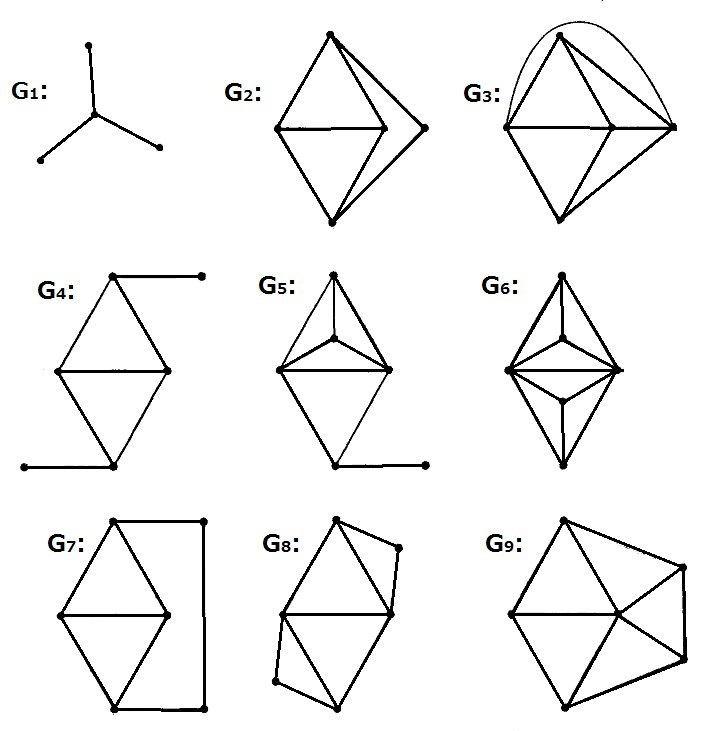
\includegraphics[scale=0.3]{nine.jpg}}
	\caption{Девять запрещённых порождённых подграфов для рёберных графов}
\end{figure}
 
\vspace{-5mm}

\begin{center}
	\subsection{Рёберные графы двудольных графов}
\end{center}

{\it Степенью} вершины $v$ в графе $G$ называется число рёбер, инцидентных~$v$.
%{\it Регулярный граф} -- граф, степени всех вершин которого равны.

\begin{theorem} \label{t8}[5]
	Если $m\ne4$ и $n\ne4$, то G -- рёберный граф полного двудольного графа $K_{m,n}$ (рис. 15) тогда и только тогда, когда 
	\\1) $G$ имеет $mn$ вершин;
	\\2) G -- регулярный граф степени $m+n-2$;
	\\3) Любые две несмежные вершины одновременно смежны точно с двумя вершинами;
	\\4) Среди смежных пар вешин точно n${m \choose 2}$ пар одновременно смежны ровно с $m-2$ вершинами, а другие m${n \choose 2}$ пар -- ровно с $n-2$ вершинами.
	
\end{theorem}

В случае $m=4=n$ существует только один граф, удовлетворяющий этим условиям и не являющийся рёберным графом графа $K_{4,4}$ [5].

Рёберный граф графа $K_{m,n}$ также можно назвать {\it ладейным графом} $(m,n)$. Он представляет допустимые ходы ладьи на доске размера $n * m$.  Вершинам графа можно задать координаты $(x,y)$,  где $1 \leq x \leq n$ и $1 \leq y \leq m$.
Две вершины $(x_1,y_1)$ и $(x_2,y_2)$ смежны тогда и только тогда, когда либо $x_1 = x_2$, либо $y_1 = y_2$, т.е. если они лежат на одной и той же линии клеток (горизонтальной или вертикальной). Мун [11] доказал, что единственным классом графов обладающим свойствами из теоремы \ref{t8}, являются ладейные графы.

%{\bf Замечание} В рёберном графе полного двудольного графа каждая вершина принаджелит двум максимальным по включению кликам.
%\\Доказательство: Т.к. каждое ребро двудольного графа $G$ принадлежит в точности двум максимальным по включению звёздам, а как не сложно заметить, рёберным графом звезды является клика. То вершины в графе $L(G)$ соответствующие рёбрам графа $G$, принадлежат в точности двум максимальным по включению кликам.

\begin{figure}
	\label{pic13.0}
	\centering{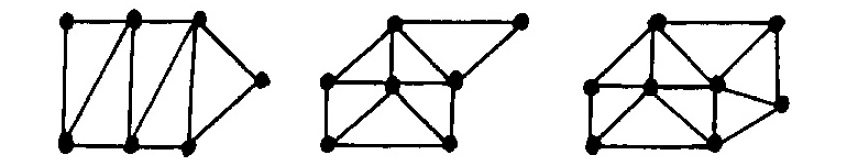
\includegraphics[scale=0.6]{3-forb.jpg}}
	\caption{Три запрещённых графа из статьи [12]}
\end{figure}

\begin{figure}
	\label{pic13}
	\centering{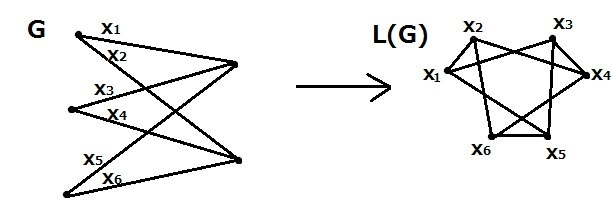
\includegraphics[scale=0.6]{dvud_reb.jpg}}
	\caption{Рёберный граф полного двудольного графа $G = K_{3,2}$}
\end{figure}
%{\it Гипотеза}: При удалении рёбер 1й клики в графе $L(G)$, которой принадлежит случайно выбранная вершина, мы получим,что такой рёберный граф получился из графа $G$ в котором было %висячих вершин столько же, сколько степень клики из которой удалили рёбра.


\begin{figure}
	\label{pic14}
	\centering{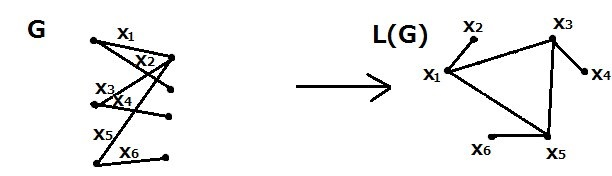
\includegraphics[scale=0.6]{dvud_reb_p.jpg}}
	\caption{Рёберный граф двудольного графа}
\end{figure}

Далее выясним, какие графы являются запрещёнными порождёнными подграфами для класса рёберных графов двудольных графов.

\begin{center}
	\subsection{Запрещённые подграфы рёберных
				 графов двудольных графов}
\end{center}

\begin{lemma}
	\label{l1}
Пусть для некоторого графа $G$ его рёберный граф $L(G)$ является простым циклом нечётной длины, не меньшей 5, без хорд. Тогда $G$ изоморфен $L(G)$, т.е. $G$ также является простым циклом нечётной длины, не меньшей 5, без хорд .
\end{lemma}
	{\bf Доказательство.} 
	Предположим противное, пусть $G$ не является простым циклом нечётной длины, не меньшей 5, без хорд. Рассмотрим граф $C$, изоморфный $L(G)$. По следствию \ref{r2} граф $L(C)$ изоморфен графу $C$, а $C$ изоморфен графу $L(G)$, значит $L(C)$ изоморфен $L(G)$. Тогда по следствию \ref{r1}, $C$ и $G$ должны быть изоморфны, противоречие. Лемма доказана.

	Помимо девяти графов, указанных в теореме \ref{t7}, в классе рёберных графов двудольных графов имеется бесконечная серия запрещённых порождённых подграфов. Эта серия описана в следующей теореме.
	
	\begin{theorem}
		\label{t10}
		В классе рёберных графов двудольных графов запрещены, в качестве порождённых, все простые циклы нечётной длины, начиная с длины 5,  без хорд.
	\end{theorem}
	{\bf Доказательство.}
	От противного, пусть $G$  произвольный двудольный граф, $L(G)$ его рёберный  граф (рис. 16). Предположим, что $L(G)$ содержит порождённый подграф $H$, являющийся простым циклом нечётной длины, не меньшей 5. %Другими словами, $H$ простой цикл без хорд нечётной длины.
	Т.к. класс рёберных графов двудольных графов является наследственным, то граф $H=L(C)$ для некоторого двудольного графа $C$. Докажем, что $C$ подграф графа $G$. Так как существует биекция между рёбрами графа $G$ и вершинами графа $L(G)$, будем удалять по ребру из графа $G$ (либо по висячей вершине с инцидентным ей ребром) и по соответствующей вершине с инцидентными ей рёбрами из графа $L(G)$. За конечное количество таких действий мы получим подграф $H$ в $L(G)$ и соответствующий ему подграф $C$ в $G$.
	\par По лемме \ref{l1}, $C$ изоморфен $H=L(C)$, т.е. $С$ является простым циклом нечётной длины, не меньшей 5, без хорд. Противоречие с теоремой \ref{t3} Кёнига. Теорема доказана.
	
	\par
	 Из теорем \ref{t7} и \ref{t10} вытекает следующее утверждение:
	 
	 \begin{result}
	\label{r3}
	В классе рёберных графов двудольных графов запрещёнными порождёнными подграфами являются  $G_1$ - $G_6$, $G_8$ (рис. 13), а также все простые нечётные циклы длины 5 и более, без хорд.
\end{result}
	\vspace{-3mm}

	\begin{theorem}
		\label{t11}
		В классе рёберных графов двудольных графов граф $K_4 - e$ является запрещённым порождённым подграфом (рис. 11).
	\end{theorem}
	{\bf Доказательство.}
	От противного, пусть $G$ произвольный двудольный граф. Предположим, что в его рёберном графе $L(G)$ содержится порождённый подграф, изоморфный $K_4 - e$. Рассмотрим все случаи, из которых мог бы получится такой подграф.
	
	Так как в графе $K_4 - e$ четыре вершины, то у породившего его подграфа $H$ в графе $G$ должно было быть 4 ребра. Причём, два из этих рёбер должны быть смежны всем рёбрам в графе $H$, так как две вершины в графе $K_4 - e$ смежны со всеми вершинами. А два оставшихся ребра не должны быть смежны друг с другом, так как две оставшиеся вершины в $K_4 - e$ не смежны друг с другом.
	
	Единственным возможным графом $H$, удовлетворяющим этим условиям, является треугольник с добавлением одной вершины, смежной только с одной вершиной из треугольника (рис. 17). Но такой граф не может являться подграфом графа $G$, так как содержит цикл длины 3. Противоречие с теоремой \ref{t3} Кёнига. Теорема доказана.
	\par
	
	Следствием теорем \ref{t10} и \ref{t11} является следующее утверждение: 
%	 \begin{result}
%	 	\label{r3}
%	 	 В классе рёберных графов двудольных графов помимо запрещённой серии указанной в теореме 10 и графа $K_{1,3}$ , запрещённым порождённым подграфом является граф $K_4 - e$.
%	 \end{result}
	 
	 \begin{theorem}
	 	\label{t12}
	 % Иными словами, теоремы 10 и 11 усиливают теорему 6 для класса рёберных графов двудольных графов, тем самым убирая графы $G2$ -- $G9$ (рис. 13) из рассмотрения.
	 В классе рёберных графов двудольных графов запрещёнными порождёнными подграфами являются $K_{1,3}, K_4 - e$ и все циклы нечётной длины, не меньшей 5, без хорд.
	\end{theorem}

Есть ли другие порождённые запрещённые подграфы для класса рёберных графов двудольных графов? В книге [7] (Corollary 7.1.4) утверждается, что других запрещённых порождённых подграфов нет. При этом авторы данного обзора ссылаются на статью [12], но в этой статье отсутствует доказательство этого факта.

	\begin{figure}
	\centering{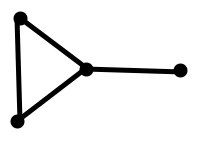
\includegraphics[scale=0.45]{triangle_with_point.jpg}}
	\caption{ Треугольник с добавлением одной вершины, смежной только с одной вершиной из треугольника}
\end{figure}

\newpage
%	\label{pic15}
%	\centering{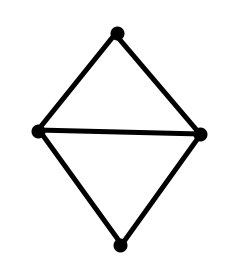
\includegraphics[scale=0.4]{K4-e.jpg}}
%	\caption{ Граф $K_4 - e$}
%\end{figure}



%	\begin{center}
%		\subsection*{Параграф}
%	\end{center}
%
%
%Наибольшее целое число $r$, при котором $K^r \subseteq  G$, называется {\it плотностью} $\omega(G)$ графа $G$, а наибольшее целое число $r$, при котором (индуцированный) $\overline{K^r} \subseteq G$, называется {\it числом независимости} $\alpha(G)$ графа $G$. Ясно, что $\alpha(G)$ = $\omega(\overline{G})$ и $\omega(G) = \alpha(\overline{G})$
%
%Граф называется {\it совершенным}, если каждый индуцированный подграф $H \subseteq G$ имеет хроматическое число $\chi(G) = \omega(G)$, т.е. если тривиальная нижняя оценка в $\omega(H)$ цветов для раскраски вершин графа $H$ не достижима.
%Таким образом, в то время как доказательство утверждения вида $\chi(G) > k$ для данного графа $G$ в общем случае может быть трудным даже в принципе, для совершенного графа оно сводится к установлению наличия подграфа $K^{k+1}$ как единственной причины нераскрашиваемости в $k$ цветов.
%
%
%	\begin{theorem} 
%		(Ловас, 1972)[5]
%	Граф является {\it совершенным}, если и только если его дополнение совершенно.
%	\end{theorem}
%	
%	Графы $G$, для которых ни $G$, ни дополнение $G$ не содержат индуцированного нечетного цикла длины не менее 5, называются {\it графами Бержа}. 
%	
%	Все совершенные графы являются графами Бержа, в силу сильной теоремы о совершенных графах.[8]
%	
%	А исходя из того соображения, что рёберные графы двудольных графов являются также графами Бержа [8], то во-первых -- в их дополнениях также запрещены нечётные циклы длины 5 и более. А во-вторых, исходя из теоремы Ловаса и Сильной теоремы о совершенных графах, дополнения к рёберным графам двудольных графов являются также совершенными графами.
%	
%	Также рёберный граф полного двудольного графа $K_{n,m}$ можно рассматривать как ладейный граф . То есть, он имеет по вершине для каждого ребра $K_{n,m}$ и две вершины ладейного графа смежны тогда и только тогда, когда соответствующие рёбра полного двудольного графа имеют общую вершину. С этой точки зрения ребро двудольного графа, соединяющее вершину $i$ одной стороны с вершиной $j$ другой стороны, соответствует клетке шахматной доски с координатами $(i,j)$.
%	
%	Любой двудольный граф является подграфом полного двудольного графа, а значит любой рёберный граф двудольного графа является порождённым подграфом ладейного графа. Рёберные графы двудольных графов совершенны — в нём и в любом его порождённом подграфе число цветов, необходимых для любой раскраски вершин, равно числу вершин в наибольшей клике. 
%	
%	Также любые две вершины полного двудольного графа принадлежат циклу длины 4.
%	
%	Рёберный граф полного двудольного графа с $p$ вершинами имеет не больше $[p^2/4]$ рёбер (Харари 32 страница).	



	\begin{center}
		\item
		\section*{Заключение}
	\end{center}

 Перечислим основные результаты дипломной работы.
 \par 1) Изучены наследственные и монотонные наследственные классы графов: леса, двудольные графы, клики, планарные графы, расщепляемые графы, кёниговы графы, блочные леса, рёберные графы. Для каждого класса приведены минимальные запрещённые подграфы.
% \par 2) Для наследственного класса рёберных графов двудольных графов было найдено, что запрещёнными порождёнными подграфами являются граф $K_4 - e$, а также бесконечное семейство порождённых запрещённых подграфов.
 \par 2) Для наследственного класса рёберных графов двудольных графов найден запрещённый порождённый подграф $K_4 - e$ и бесконечное семейство порождённых запрещённых подграфов -- циклов нечётной длины, не меньшей 5.
  
 \newpage
  
\begin{center}
	\item
	\subsection*{Список литературы}
\end{center}

1. Алексеев В.Е., Замараев  В.А., Захарова Д.В., Малышев Д.С., Мокеев Д.Б. Некоторые результаты о наследственных классах графов // Вестник Нижегородского университета им. Н.И. Лобачевского. 2011. N 6 (1). С. 169–173.

2. Алексеев В.Е., Захарова Д.В., Малышев Д.С., Мокеев Д.Б., Сорочан С.В. Некоторые результаты о наследственных классах графов II // Вестник Нижегородского университета им. Н.И. Лобачевского. 2012. N 6 (1). С. 115–120.

3. Алексеев В.Е., Замараев  В.А., Захарова Д.В., Малышев Д.С., Мокеев Д.Б., Сорочан С.В. Некоторые результаты о наследственных классах графов III // Вестник Нижегородского университета им. Н.И. Лобачевского. 2013, N.6 (1). С. 165–172.

4. Дистель Р. Теория графов. Новосибирск: Издательство ИМ СО РАН, 2002.

5. Харари Ф. Теория графов. М.: Мир, 1973.

6. Bandelt H.J., Mulder, H. M. Distance-hereditary graphs // J. Comb. Theory, Ser. B. 1986. V. 41, No.2. P. 182–208.

7. Brandstaedt A., Le V.B., Spinrad J. Graph classes: A survey. SIAM Monographs on Discrete Mathematics and Applications. Society for Industrial and Applied Mathematics, 1999.

8. Chudnovsky M., Robertson N., Seymour P., Thomas R. The strong perfect graph theorem // Annals of Mathematics. 2006. V. 164, No.1. P. 51–229.
 %Mackenzie, Dana (July 5, 2002), "Mathematics: Graph theory uncovers the roots of perfection", Science, 297 (5578): 38.

9. Golumbic M.C. Algorithmic Graph Theory and Perfect Graphs. NY University, Courant Institute of Mathematical Sciences, 1980.
% Theorem 6.3, p. 151.

10. Maurer S.B. Matroid basis graphs I // J. Combin. Theory. Ser. B. 1973. V. 14, No. 1. P. 216-240

11. Moon J. W. On the line-graph of the complete bigraph // Annals of Mathematical Statistics. 1963. V. 34, No. 2. P. 664—667.

12. Soltes L. Forbidden induced subgraphs for line graphs // Discrete Mathematics 132, P. 391-394. Department of Mathematics, CHTF Slovak Technical University, Bratislava, Czechoslovakia, 1994.


\end{document}

